\newpage
%%%%%%%%%%%%%%%%%%%%%%%%%%%%%%%%%%%%%%%%%%%%%%%%%%%%%%%%%%
%%%%%%%%%%%%%%%%%%%%%%%%%%%%%%%%%%%%%%%%%%%%%%%%%%%%%%%%%%
\section{Review of Theory}
\label{review:pim-theory-review}
%%%%%%%%%%%%%%%%%%%%%%%%%%%%%%%%%%%%%%%%%%%%%%%%%%%%%%%%%%
%%%%%%%%%%%%%%%%%%%%%%%%%%%%%%%%%%%%%%%%%%%%%%%%%%%%%%%%%%
%%%%%%%%%%%%%%%
% SIGNPOSTING
%%%%%%%%%%%%%%%
% \textbf{Section~\ref{review:pim-research-overview}} identified two main areas of substantive research concerned with personal information management: empirical studies and technology design. This section reviews theoretical work in the area, identifies a lack of progress, and suggests approaches which might be applied in the future.
% What theory has been done?
% What theoretical methods could be applied?
%%%%%%%%%%%%%%%%%%%%%%%%%%%%%%%%%%%%%%%%%%%%%%
%% Why theory? -- HCI in general
%%%%%%%%%%%%%%%%%%%%%%%%%%%%%%%%%%%%%%%%%%%%%%%
%% focus on application of theory to design as the ideal. 
%% Newman: To explain what it is/How it works, allow prediction of design utility, to give principled advice to designers.
% Firstly the place of theory within HCI is discussed. Rogers~
% More specifically what can it offer to the study of PIM? How can theory help PIM designers? 
This section surveys theoretical work on PIM that is relevant to this thesis.  \citet{rogers:04} presents four aims of theory within HCI: to describe interactive phenomena, to explain interactive phenomena, to make predictions of the output of a design (e.g. in terms of user performance), and to generate new routes for design.

%%%%%%%%%%%%%%%%%%%%%%%%%%%%%%%%%%%%%%%%%%%%%%
%% Focus on integration
%%%%%%%%%%%%%%%%%%%%%%%%%%%%%%%%%%%%%%%%%%%%%%%
% The particular aim in this thesis to to systematically investigate the promise of improving integration between PIM-tools. This chapter surveys theory relevant to personal information management in general, but application to the exact research problem of PIM-integration is of prime consideration.
%%%%%%%%%%%%%%%%%%%%%%%%
% Overview of survey
%%%%%%%%%%%%%%%%%%%%%%%%
%%%%%%%%%%%%%%%%%%%%%%%%%%%%%%%%%%%%%%
%% THINK: structuring of survey
%%%%%%%%%%%%%%%%%%%%%%%%%%%%%%%%%%%%%%%%%%%%%%%%%%%%%%%%%%%%%%%%%%%%%%%%%%
%% * THINK: divide up by cognitive level/tool/aspect of PIM/type of user?
%% * Include empirically-driven theory and models here?.
%%%%%%%%%%%%%%%%%%%%%%%%%%%%%%%%%%%%%%%%%%%%%%%%%%%%%%%%%%%%%%%%%%%%%%%%%%
% The remainder of this section surveys relevant bodies of theory. 
% \textbf{Section~\ref{review:theory-foundations}} provides an overview of foundational theory from cognitive psychology and classification research. Then, 
% Later sections survey , and describe criticisms that have been levelled at hierarchical forms of organization. % , and also the potential of descriptive frameworks such as Activity Theory for use in this area.
The section is structured as follows. Firstly, \textbf{Section~\ref{review:theory-pimmodels}} considers descriptive and predictive models of PIM.  \textbf{Section~\ref{review:theory-pimmodels:ir}} then briefly discusses two models of information retrieval. \textbf{Section~\ref{review:theory-classificationschemes}} discusses the theory of personal classification, and critiques that have been levelled against the folder hierarchy.


%%%%%%%%%%%%%%%%%%%%%%%%%%%%%%%%%
% Refer to theory in Chapter 2
%%%%%%%%%%%%%%%%%%%%%%%%%%%%%%%%%
% The reader should refer to the high-level descriptive theory surveyed in Chapter 2, such as the high-level task decomposition of personal information management in
%% Basic PIM intro stuff in Chapter 2 (e.g. Break-down by Barreau~\citep{barreau:95}), criticism of the hierarchy}
% A number of definitions of PIM were discussed in \textbf{Chapter~\ref{chapter:bg}}, in particular Barreau's analysis of PIM into component sub-activities~\citep{barreau:95}.




%%%%%%%%%%%%%%%%%%%%%%%%%%%%%%%%%%%%%%%%%%%%%%%%%%%%%%%%%%%
\subsection{Models of Personal Information Management}
\label{review:theory-pimmodels}
%%%%%%%%%%%%%%%%%%%%%%%%%%%%%%%%%%%%%%%%%%%%%%%%%%%%%%%%%%%
%% THINK: relate to particular aspects of PIM?}
This section surveys two types of model that have been proposed: (1) descriptive models that do not attempt to make predictions of user behaviour, and (2) predictive models of user behaviour that can be used to issue prescriptive advice to direct design.

%%%%%%%%%%%%%%%%%%%%%%%%%%%%%%%%%%%%%
\subsubsection{Descriptive Models}
\label{review:theory-pimmodels:descriptive}
%%%%%%%%%%%%%%%%%%%%%%%%%%%%%%%%%%%%%

%%%%%%%%%%%%%%%%%%%%%%%
% DESCRIPTIVE MODELS
%%%%%%%%%%%%%%%%%%%%%%%
Earlier sections of this thesis have covered areas of descriptive theory.  These include Barreau's conceptual framework of PIM sub-activities~\citep{barreau:95}, and classifications of organizing strategies in PIM-tools such as email, e.g.~\citep{Whittaker-email:96}.  %  in which she identifies four sub-activities that make up personal information management. See \textbf{Chapter 2} for more discussion. % Closer to a task description?
%% need to expand here? Should I even mention descriptive models such as this?

As noted in \textbf{Section~\ref{review:pim-empirical-review}}, few empirical studies have captured data on PIM over time.  However, based on classifications of email management strategies, Balter proposes a model representing possible strategy changes over time~\citep{ob:97}.  The model is summarized in \textbf{Figure~\ref{fig:ch2_balter_model}}, and can be can be summarized in terms of two sets of strategy transitions.  These can be described as ``\textit{pro-organizing}'' transitions (solid lines), and ``\textit{anti-organizing}'' transitions (dashed lines).  Balter suggests that under the pressure of increasing information overload, many users may follow the ``anti-organizing'' transitions and become less reliant on filing over time. He proposes that folderless spring-cleaner may be an optimizing ``end-state'' for many users who receive large numbers of email. Other users may instead choose to devote increased effort towards management and move the other way (e.g. from spring-cleaner to frequent-filer). He observes that further longitudinal data is required to confirm his model. 

% %%%%%%%%%%%%%%%%%%%%%%%%%%%%%%%%%
% FIGURE - Balter's longitudinal model
%%%%%%%%%%%%%%%%%%%%%%%%%%%%%%%%%%%
\begin{figure}[hbtp]
	\begin{center}
		\leavevmode	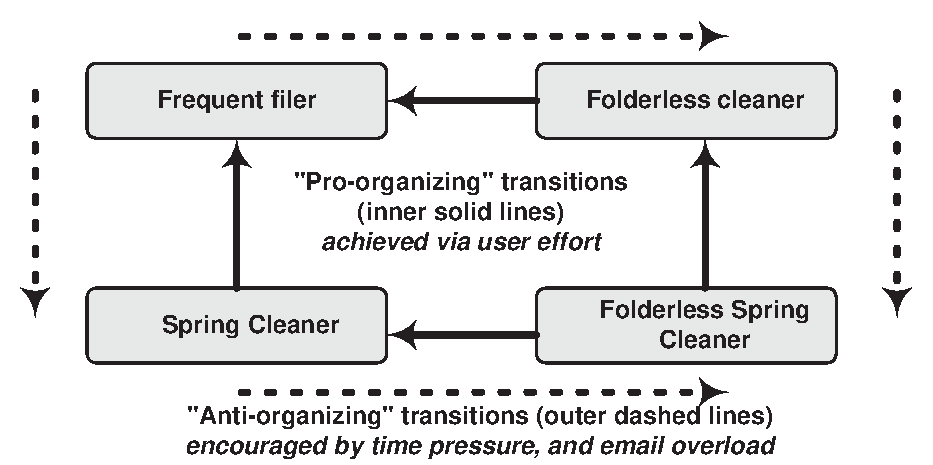
\includegraphics[width=.7\textwidth]{pictures/research_review/Ch2-BalterLongitudinalModel.pdf}
	\end{center}
	\caption{Model of changes in email management strategy over time~\citep{ob:97}}
	\label{fig:ch2_balter_model}
\end{figure}


%%%%%%%%%%%%%%%%%%%%%%%%%%%%%%%%%%%%%%
% \subsection{Descriptive Frameworks}
%%%%%%%%%%%%%%%%%%%%%%%%%%%%%%%%%%%%%%
%% Refer to as descriptive frameworks?
%% Highlight import of context, and information is used? 
% Trends in HCI theory have been described as a \textit{turn towards the social}~\citep{rogers:04}. Several theoretical methods, heavily influenced from sociology have been taken up by HCI researchers including Distributed Cognition and Activity Theory.
%%%%%%%%%%%%%%%%%%%%%%%%%%%
% DISTRIBUTED COGNITION
%%%%%%%%%%%%%%%%%%%%%%%%%%%
Distributed Cognition (DC) is a theoretical framework which has been used to model cognitive processes distributed across time, space and multiple actors, e.g. aircraft carrier control rooms~\citep{dc:00}.
%%%%%%%
% DIX
%%%%%%%
Two sets of descriptive terminology have been proposed to describe the functions provided by items and tools in the user's personal information environment.  \citet{dix:98} offers a conceptual framework describing the function of items in supporting user activities.  He identifies two key concepts: (1) \textit{triggers}, items such as reminders that can initiate action, and (2) \textit{placeholders} which are arrangements of items which can maintain task state allowing it to be restarted at a later time.  A second, more abstract set of terminology is offered by~\citet{dk:01}.  Kirsh reports a theoretical analysis of an information environment as an activity space within which the user carries out their tasks.  He proposes a number of theoretical constructs to describe the conceptual structures that users project onto the environment: (1) \textit{entry points} (cues to start tasks), (2) action landscapes (arrangements of items that support a particular activity), and (3) coordinating mechanisms (artefacts such as calendars that allow the user to perform multiple activities).  \citet{Whittaker-rta:00} note the need for the community to agree on standardized descriptive terminology as a stepping stone to developing predictive theories.  The above frameworks represent the first steps towards establishing agreed terminology in this area.  % although at an early stage of development, represent important progress in this direction.  

% However it is not clear how such descriptive frameworks would be applicable to design and would probably suffice as a stepping stone towards further research.
% offers a theoretical analysis of PIM, considering the PIM-system as distributed between an individual and their environment. Kirsh describes how user and their PIM environment co-evolve over time, and 
%%%%%%%%%%%%%%%%%%%%%%%%%%%%%%%%%%%%%%%%%%%%%%%%%%
% Existing theory is focused on storage+retrieval
%%%%%%%%%%%%%%%%%%%%%%%%%%%%%%%%%%%%%%%%%%%%%%%%%%
% Current task descriptions of PIM are focused on the traditional perspective of storage for future retrieval. There is also a need for theory to handle contextualizing functions of personal information management such as reminders, and task management.

%%%%%%%%%%%%%%%%
% KAPTELININ
%%%%%%%%%%%%%%%%
% Activity Theory -- A conceptual framework, not predictive or cookbook in terms of design. Basic principles: object relatedness, hierarchical structure of activity (activities (motives), actions (goals), operations (conditions)), internalization/externalization, mediation, development.
% \citep{Kaptelinin:03} applies an another theoretical framework to PIM: Activity Theory~\citep{bn-at:95}. He performs an analysis of a user's activities in which personal information is used. The theoretical analysis is used to provide design rationale for the \textit{UMEA} system.
% Distributed Cognition and Activity Theory may prove useful as conceptual frameworks to define a descriptive vocabulary for personal information management. 



%%%%%%%%%%%%%%%%%%%%%%%%%%%%%%%%%%%%%
\subsubsection{Predictive Models}
\label{review:theory-pimmodels-predictive}
%%%%%%%%%%%%%%%%%%%%%%%%%%%%%%%%%%%%%
% However, two models of email usage have been proposed. \citet{Whittaker-email:96} propose a simple \textit{one-touch} model of inbox processing: that items are opened, read and then immediately filed or deleted.  They acknowledge that this is inaccurate since studies, including their own observe users keeping many messages for later processing.
%%%%%%%%%%%%%%%%%%%%%%%
% PREDICTIVE MODELS
%%%%%%%%%%%%%%%%%%%%%%%
% However his findings have been countered by recent empirical findings that suggest that many experienced users develop , a strategy which Balter indicates is inefficient. % The model can be criticised for not encompassing filters and other realistic aspects of information management.
% Furthermore, the model relies of . Users will expend more time and effort storing information which is highly valued. It is therefore in their interest to structure the information environment so as to make frequently accessed information easy to find.  The question remains can purely economic considerations be used to predict user behaviour. All these models are founded on the premise that information is stored for later retrieval. Other aspects of information management such as reminding are not encompassed.
Few predictive models of PIM behaviour have been developed.  One exception is that of \citet{ob:00} who proposes a keystroke-level model of email archiving and retrieval.  Based on the model, Balter issues prescriptive advice to tool designers and to users with respect to optimizing their behaviour in terms of time efficiency.  Balter's model can be criticised for its reliance on economic costs of information access and storage.  For example, one of Balter's claims is that any strategy involving more than 30 folders is inefficient.  Studies of email usage have observed highly experienced email users with large numbers of folders~\citep{Ducheneaut:01}.  Such findings suggest that either Balter's model is inaccurate, or that there is more at stake than time efficiency in dictating choice of management strategy.  Factors such as the need for tidiness, or the placement of items as reminders are not captured within the model.  However, Balter's work should be acknowledged as a first step in generating prescriptive advice in this complex area.

%%%%%%%%%%
% PAYNE
%%%%%%%%%%
% Payne~\citep{sp:93} carried out a cognitive-artifact analysis on personal calendar usage. He observed how people employ multiple calendar artefacts but typically rely on paper calendars. Payne states that electronic calendars, even though often used for collaborative scheduling, should be treated by developers as personal artefacts.


%%%%%%%%%%%%%%%%%%%%%%%%%%%%%%%%%%%%%%%%%%%%%%%%%%%%%%%%%%%%%%%%%
%% Typical criticism:  use to illustrate research-practice gap}
%%%%%%%%%%%%%%%%%%%%%%%%%%%%%%%%%%%%%%%%%%%%%%%%%%%%%%%%%%%%%%%%%

%%%%%%%%%%%%%%%%%%%%%%%%%%%%%%%%%%%%%%%%%%%%%%%
\subsection{Models of Information Retrieval}
\label{review:theory-pimmodels:ir}
%%%%%%%%%%%%%%%%%%%%%%%%%%%%%%%%%%%%%%%%%%%%%%%
% Other references - see Weiss-Lijn thesis
%%%%%%%%%%%%%%%%%%%%%%%%%%%%%%%%%%%%%%%%%%%%%%%

%%%%%%%%%%%%%%%%%%%%%%%%%%%%%%%%%%%%%%%%%%
% general intro on information retrieval
%%%%%%%%%%%%%%%%%%%%%%%%%%%%%%%%%%%%%%%%%%
% (AKA information-seeking or information-foraging) 
\textbf{Section~\ref{bg:pim-relatedterms}} highlighted how information retrieval is a key aspect of PIM.  Theories from information retrieval may be useful to the developers of more general PIM-related theories.

% Firstly, it relates to the retrieval of items from a user's PIM system. Secondly it relates to the retrieval of information from remote information systems to include in a user's PIM system. An example of this would be downloading a document from the web and saving a local copy. \textbf{Section\ref{bg:pim-relatedterms}} discusses the relationship between information retrieval and personal information management.
%%
%% relate to earlier discussion on relationship between PIM and other areas}. Reference diagram. 
%%
% As such information retrieval should be considered as a lower-level process than personal information management, but one which is complex in itself. An information retrieval system has been defined as \textit{an information retrieval system does not inform (i.e. change the knowledge of) the user on the subject of his inquiry. It merely informs on the existence (or non-existence) and whereabouts of documents relating to his request}~\citep{Rijsbergen:79}. Information retrieval is guided by the notion of an information need. The ongoing process of PIM will encompass many distinct information retrieval events.
%% 
%% IR lower level than PIM -- one aspect of PIM, also focus has mainly been GIS rather than PIS. But NB: complex in itself.
%%%%%%%%%%%%%%%%%%%%
% USeful for PIM
%%%%%%%%%%%%%%%%%%%%
% Information retrieval is a field with its own conferences and journals and is generally much more mature than personal information management. Reasons for this are discussed below. Theories from information retrieval may be useful to the developers of PIM-systems. Examples are discussed below.


%%%%%%%%%%%%%%%%%%%%%%%%%%%%
% information foraging
%%%%%%%%%%%%%%%%%%%%%%%%%%%%

\textit{Information Foraging (IF)}~\citep{pirolli:99} is a theory that supports the construction of computational models of information-seeking behaviour.  The theory is based on evolutionary theories of survival, leading to the premise \textit{``that information systems evolve towards a stable state of maximising the transfer of valuable information per unit cost''}.  Users will seek to follow an optimal strategy so as to achieve this.  Three activities are considered: (1) enrichment, (2) scent following, and (3) exploitation.
% NB: users won't necessarily follow an optimal strategy though
The models encompasses a notion of information value in terms of information scent, and the cost of interaction (e.g. mouse clicks). % The ACT-IF model has been used to simulate behaviour in a scatter/gather prototype.
IF theory has been most recently applied to website design.


%%%%%%%%%%%%%%
% Sutcliffe
%%%%%%%%%%%%%%
% An alternative approach is employed by Ennis \& Sutcliffe~\citep{sutcliffe:98} who present a cognitive model of information retrieval



%%%%%%%%%%%%%%%%%%%%%%%%%%%%%%%%%%%%%%%%%%%%%%
% \subsection{Models of Information behaviour}
%%%%%%%%%%%%%%%%%%%%%%%%%%%%%%%%%%%%%%%%%%%%%%
% Generally information science has been more focused on information retrieval than other aspects of PIM.
% Wilson criticises this over-focus and presents a more encompassing theory of information behaviour. This is discussed in the next section.
% which is typically left unspecified in the information retrieval literature.
\citet{wilson:99} observes that many models of information retrieval do not encompass how that information is used, beyond the general notion of an \textit{information need}.  He proposes a general model of information behaviour that encompasses information retrieval and other aspects of information usage.  However, the model does not capture aspects of PIM such as how information may be stored and organized over time.








%%%%%%%%%%%%%%%%%%%%%%%%%%%%%%%%%%%%%%%%%%%%%%%%
\subsection{Personal Classification Schemes}
\label{review:theory-classificationschemes}
%%%%%%%%%%%%%%%%%%%%%%%%%%%%%%%%%%%%%%%%%%%%%%%%

%%%%%%%%%%%%%%%%%%%%%%%%%%%%%%%
% Studies of classification
%%%%%%%%%%%%%%%%%%%%%%%%%%%%%%%
%%%%%%%%%%%%%%%%%%%%%%%%%%%%%%%%%%%%%%%%%%%%%%
%% Other stuff from classification science
%%%%%%%%%%%%%%%%%%%%%%%%%%%%%%%%%%%%%%%%%%%%%%
%% Personal versus Shared ontologies~\citep{shapiro:99}. Messes~\citep{abrahamson:02}
%% Has it been applied? 
% , a cognitive process that is applied during the organizing material in semantic or spatial categories.
% Borges~\citep{borges:62} highlights the need for classification -- to deal with the complexity of the world (cognitive economy).  
% The second relevant body of basic science relates to the cognitive process of classification.. Cognitive psychology and classification science offer many findings on the workings of human classification processes.
\textbf{Chapter~\ref{chapter:bg}} noted that most current PIM-tools are centred on a hierarchical classification mechanism.  This section surveys some theory on classification, before describing criticisms that have been levelled at the folder hierarchy.

The folder hierarchy allows the user to specify a classification scheme within which items can be categorized. \citet{bs:99} define a classification scheme as \textit{``a spatial, temporal or spatio-temporal segmentation of the world''}. They propose three theoretical properties of a classification scheme: (1) a consistent, unique classificatory principle, such as temporal or alphabetical ordering, (2) mutually exclusive categories, and (3) completeness. However, as they note, no real-world classification is this ideal -- classificatory principles often contradict, categories overlap, and many items cannot be categorized (hence the use of catch-all categories such as ``stuff'').

Many theories of classification have been developed through the ages. The Classical Theory originated with Plato in Ancient Greece~\citep{ek:90}.  
%% summarised in Margolis and Laurence 1999.
The Classical Theory states that the cognitive concepts on which categories are based carry their own definitional structure. Categorizing an item is thus the process of matching its features against those of the concept. In recent years the Classical Theory has been subjected to intense criticism, and other views such as Prototype Theory~\citep{er:78} have come to the fore. Prototype Theory states that a category is a statistical representation of the
properties that its members tend to have, i.e. each category is represented by an exemplar. Under Prototype Theory, categorizing an item involves comparing it to each category's exemplar. Rosch identifies two basic principles that influence the formation of categories: (1) cognitive economy (classification is about providing maximum information about the world for the least cognitive effort), and (2) perceived world structure (categories are based on the high correlational structure possessed by the attributes of real-world objects).  These two principles have implications for the level of abstraction of categories formed in a category system (inclusiveness), and the internal structure of those categories once formed (prototypes).

Classification schemes can be considered as a means of cognitive scaffolding~\citep{jacob:01} -- they allow people to deal with the complexity of large systems. % Jacob identifies two types of classification scheme: personal and infrastructural. Infrastructural classification schemes are developed by an organization or society, whilst personal classification schemes are developed by an individual.
%% ADD EXAMPLE
%% YUCK - TIDY THIS
~\cite{ob:00} describes the retrieval-time benefits from organizing in terms of "reducing the search space". Instead of scanning a long list of unstructured items, users can home in on a particular subset directly.

% In contrast to pre-defined structures, a personal classification scheme allows the user to create an individualised organization, customized to their way of thinking and working. The user may choose to create categories based on whichever organisational dimensions  that they see as relevant (e.g. role, project or time). Categories can be represented in various ways, depending on the classificatory mechanism in use.  A typical desktop workspace might contain categories in the form of a cluster of icons at a spatial location, emails contained within a folder labelled semantically with a text string, or a set of hypertext links on a personal web page.

% Our electronic workspaces contain a wide range of personal classification schemes. Common examples in desktop workspace include the folder hierarchies of the file system, mail tools and web browsers for organising documents, messages and web links respectively. Resources may also be organized spatially as an arrangement of icons on the desktop. Many software packages also contain their own specific hierarchies for organising specialized types of informationsuch as source code, images and music files. Some operating systems contain their own idiosyncratic hierarchies, such as the Start Menu of Microsoft Windows that is used to organise software tools and access recently accessed documents. Workspace itself may be organized in terms of virtual windows assigned to a flat category space~\cite{rooms:86}.

%%%%%%%%%%%%%%%%%%%%%%%%%%%%%%%%%%%%%%%
% HOW TO APPLY TO REAL-WORLD DESIGN?
%%%%%%%%%%%%%%%%%%%%%%%%%%%%%%%%%%%%%%%
%%  not really theory of PIM but provide foundation for much of the design work.
%% How have findings been used? Have any been used beyond general ad-hoc scientific grounding
% The question remains over whether findings from objective lab studies relating to low-level cognitive processes involved in personal information management such as recall, recognition and classification can offer useful guidance for designers developing tools for use in the real world.  % Lansdale~\citep{ml:92} makes design suggestions drawn from the basic findings such as providing the user with multiple retrieval cues.
% However, it not clear how such low-level principles can be made relevant to designers.  The research has been useful however in terms of documenting the basic cognitive capabilities of users.    

			
%%%%%%%%%%%%%%%%%%%%%%%%%%%%%%%%%%%%%%%%%%%%%%%%%%%%
\subsubsection{Limitations of the Folder Hierarchy}
%%%%%%%%%%%%%%%%%%%%%%%%%%%%%%%%%%%%%%%%%%%%%%%%%%%%%
%%%%%%%%%%%%%%%%%%%%%%%%%%%%%%%%%%%%%%%
%% Rationalize with stuff in Chapter 2
%% Is this designer intuition or actual theory?
%%%%%%%%%%%%%%%%%%%%%%%%%%%%%%%%%%%%%%%
%% Also: Ad-hoc categories.
%% Limits of such anecdotal commenary. NB: usually accompanies non-evaluated revolutionary prototype.
% Many research prototypes have been motivated by intuitive technological arguments.
Hierarchies are the standard computational mechanism used to define personal classification schemes~\citep{dourish:99a}. They are both easy to program and familiar to most users. However, 
a number of criticisms have been levelled at the hierarchy, e.g. ~\citep{nielsen:96,bell:02,tn:99,Gelernter:96a,dourish:99a,jr:00}
\footnote{Similar arguments against hierarchical schemes have also been made in other domains such as architecture. \citet{alexander:65} argues that a hierarchical city layout is not a good match for the dynamic and interleaved nature of human activity.}.
One fundamental limitation is that of \textit{single-inheritance}~\citep{nielsen:96,dourish:99a}, i.e. an item may only be filed in one place. Most operating systems provide mechanisms to override single-inheritance in
the form of links (UNIX), aliases (MacOS) or short-cuts (Windows) but they often confuse users~\citep{dourish:99a}. Furthermore, hierarchies have also been criticized for their static nature, and for poor scalability to large information spaces.

%% ADD THE FOLLOWING BACK IN?
%% Structuring items into categories also impedes the use of implicit
%metadata. Chronological information is an example of a organizing principle
%often used by individuals to organize various types of personal information
%such as bookmarks and email. 


%%%%%%%%%%%%%%%%%%%%%
% DEFENSE OF TREE
%%%%%%%%%%%%%%%%%%%%%	
% Further discussion is provided in \textbf{Section~\ref{bg:pimtool-cf}}.
%% CHECK THIS 
%% Large amount of non-rigorous (mainly) insubstantiated postering. Attack and (little) defense of the hierarchy.	  Summarize main points
%% Interject with defense of the tree here? Why is the tree so dominant?
%% Andy Hertzfeld quote -- tree as totally fundamental
%% Add \textbf{Claims analysis} of the tree?
The question of why the traditional folder hierarchy continues to dominate PIM-systems is an interesting one.  Alternatives offering more flexibility have been available for over a decade, e.g.~\citep{semanticfs:91}.  The key technological advantage of the tree is that it is simple and easy to implement.  Although the above criticisms have had a profound influence in design, questions remain over whether they are confirmed by user data.  For instance, ~\citet{bn:95} report that the participants in their study were satisfied with their folder organizations and had little need for multiple classification. This suggests that the hierarchy, despite its limitations, has the benefits of being an organizational paradigm which users are broadly satisfied and familiar with. % Also it offers a positive constraint of knowledge domain and participant~\citep{jacob:01}, persistence, and the ability to assign multi-attributes in one go.






%%%%%%%%%%%%%%%%%%%%%%%%%%%%%%%%%%%%%%%%%%%%%%%%%%%%%%%%%%%%%%%%%%%%%%%
\subsection{Discussion of Theoretical Contributions}
\label{theoretical-contribution-discussion}
%%%%%%%%%%%%%%%%%%%%%%%%%%%%%%%%%%%%%%%%%%%%%%%%%%%%%%%%%%%%%%%%%%%%%%%
%%%%%%%%%%%%%%%%%%%%%%%%%%%%%%%%%%%%%%%%%
% WHY DO WE WANT THEORY ANYWAY?
%%%%%%%%%%%%%%%%%%%%%%%%%%%%%%%%%%%%%%%%%
% What would such theory be useful for? 
% Theoretical discussions and models (can they explain data?) -- types of theory: descriptive, explanatory, prescriptive, generative etc. Lack of encompassing theory and frameworks
% Newman:  Why not appropriate for PIM tools? 
%%%%%%%%%%%%%%%%%%%%%%%%%%%%%%%%%%%%%%%%
% Issue: how to be useful for design
%%%%%%%%%%%%%%%%%%%%%%%%%%%%%%%%%%%%%%%%
%% Key issues: applicability, scalability.
%% Retouch the Theory/Practice Gap
% Too low-level: other cognitive models. Why?~\citep{ml:92}
% Medium-level but not relevant: information-seeking, information-foraging
% Too high-level: descriptive frameworks. Consider use of AT as an approach.


%%%%%%%%%%%%%%%%%
% BOTTOM LINE
%%%%%%%%%%%%%%%%%
% Theory tends to work at the extremes: low-level cognitive phenomena, or high-level collaborative scale
% Bodies of theory are identified from other areas which may be applicable. 
% there is a lack of coherenmt theory of PIM.  Instead, 
% no coherent theory of PIM. In general theory tends to be very low-level (cognitive scale) or very high-level (descriptive theory).
This section confirms the observation of \citet{Whittaker-rta:00}, that there is a lack of theoretical foundation for PIM, despite its status as a fundamental computer-based activity.  % A range of theoretical work to PIM has been surveyed. 

\citet{Whittaker-rta:00} highlight the need for standardized descriptive vocabulary as a first step towards developing more powerful predictive theories that can provide principled advice to designers, and dictate design characteristics.  Conceptual frameworks such as those described in \textbf{Section~\ref{review:theory-pimmodels}}, have made some progress in this area, but there is clearly much more to be done.
% , there is 
% Theory from information retrieval could for example be applied to model retrieval from personal information management systems. However some higher-level framework is required to tie retrieval and storage together, along with acquisition and maintenance.

% \textit{A ``devils advocate'' argument is provided by advocates of the empiricist perspective on HCI  (Landauer etc.): that much HCI behaviour is too complex to predict/design from theory. Instead, they advocate  use alternative of iterative requirements-gathering, design and evaluation and treat designed artefacts as theory~\citep{Carroll-cycle:91}.} % This perspective on HCI theory is discussed in more detail in \textbf{Section~\ref{hci-state}}.

\citet{rogers:04} outlines a number of properties of effective HCI theories, that highlight the kind of theory needed in this area.   Firstly, the theory should \textit{scale} to an appropriate granularity of task.  However, much HCI theory is focused at a low-level on the cognitive, perceptual, and motor function systems~\citep{newman:95}.  In the context of PIM, cognitive theories of human memory and classification may not be applicable to  modelling natural real-world classification decisions in a hectic work environment~\citep{ml:92}. Other theory is very high-level, such as the conceptual frameworks offered by~\citet{dk:01}.  One route may be to combine theories which focus on different levels of analysis~\citep{barnard:00}.   Secondly, theory must be \textit{applicable}.   The challenge for theorists is to develop models that can be useful in a design context.  It is not clear how much of the existing body of theoretical work is of practical help to designers.
% A meta-theory could try and relate low-level cognitive processes involved in one-off storage and retrieval decisions (medium-level) to other high-level long-term user activities.


%%%%%%%%%%%%%%%%%%%%%%%%%%%%%%%%%%%%%%%%%%%%
% Relevance to integration in particular
%%%%%%%%%%%%%%%%%%%%%%%%%%%%%%%%%%%%%%%%%%%%
% Since there is no theory applicable to a single PIM-system, it follows that there is none relevant to inter-tool integration. A first step may be to develop appropriate descriptive vocabulary. Whittaker \textit{et al}.~\citep{Whittaker-rta:00} argue that for effective theory-building you first need more empirical groundwork to achieve consensus on task description, and descriptive vocabulary.

% Little theory exists that is directly applicable to PIM-integration/unification.
% No coverage in particular of issues relating to multiple tools and integration.


%%%%%%%%%%%%%%%%%%%%%%%%%%%%%%%%%%%
% Alternative approach to theory
%%%%%%%%%%%%%%%%%%%%%%%%%%%%%%%%%%%
% May be a better approach since so much design out there in the real world. Create theory to establish why these tools work as well as they do. And furthermore a theoretical baseline for dealing with observed problems.

% %%%%%%%%%%%%%%%%%%%%%%%%%%%%%%%%%
% FIGURE - Coverage of Theories
%%%%%%%%%%%%%%%%%%%%%%%%%%%%%%%%%%%
% \begin{figure}[t]
%	\begin{center}
%		\leavevmode
%		
\includegraphics[height=2in, width=.9 \textwidth]{pictures/research_review/Ch2-TheoryCoverage.pdf}
%	\end{center}
%	\caption{Coverage of theories}
%	\label{fig:chapter2_theory_coverage}
%\end{figure}

	
%%%%%%%%%%%%%%%%%%%%%%%%%%%%%%%%%%%%%
%% \subsubsection{Directions for future theoretical research}
%%%%%%%%%%%%%%%%%%%%%%%%%%%%%%%%%%%%%%

%%%%%%%%%%%%%%
% SIGNPOSTING
%%%%%%%%%%%%%%%
% This section reviewed the third research area identified in \textbf{Section~\ref{review:pim-research-overview}}: theory relevant to PIM software. It is concluded that little theory exists in the area for design guidance. Some basic theory can be built on in terms of developing a descriptive framework. The next section draws together work presented in this section and the two previous ones to present a view on the overall state of research concerned with personal information management.



%%%%%%%%%%%%%%%%%%%%%%%%%%%%%%%%%%%
%%%%%%%%%%%%%%%%%%%%%%%%%%%%%%%%%%%
%%%%%%%%%%%%%%%%%%%%%%%%%%%%%%%%%%%
%%%%%%%%%%%%%%%%%%%%%%%%%%%%%%%%%%%